\chapter{Advanced}
\label{cha:Advanced}
This section of the help document outlines the app's advanced features. These functionalities are all available through the "Advanced" option in the top menu.

\section{Batch analysis}
Batch analysis offers an automated way of analyzing all the spectra in the selected folder. For using this functionality, just load one spectrum, select the desired range of analysis, and build/load the appropriate model.

Following the execution of the Batch analysis, the application simply requests the format of the spectrum files it will process and the directory where they are located. It then proceeds to analyze each file in the folder, using the same boundaries as the spectrum used to build the model, optimizing the model parameters, and storing the images in a subfolder within the chosen directory. Once all spectra have been fitted, the optimized parameter values and their errors are documented in an Excel file within the same subfolder.

\section{1D mapping}

One-dimensional (1D) Raman mapping refers to the analysis of spectral evolution as a function of a single varying parameter. In the context of this application, 1D maps are typically acquired by recording Raman spectra sequentially while changing an external variable, such as electrochemical \textbf{potential}, elapsed \textbf{time}, or \textbf{position} along a linear spatial scan.

This type of analysis enables users to monitor dynamic changes in materials, detect chemical or structural gradients, and track reaction progress over time or space. The app supports the import, visualization, and automated processing of 1D datasets in a user-friendly format designed to allow efficient exploration of such trends.

Currently, this app is capable of importing only 1D files, specifically those from Horiba .txt files that have been exported as "split" arrays. To export the timemap and line scans in this format, navigate to the save button in the LabSpec6 software, click the small arrow next to it, and select the "Split array" option. This will automatically export the map into separate files, including time or distance information in both the filename and the file header. For potential maps (SEC - SpectroElectroChemistry), the files must include the potential values applied to the working electrode during spectrum acquisition, with mV as the locator string for reading the potential. For example, a filename such as \textit{$sample\_12\_-800mV.txt$} indicates a spectrum recorded at -800 mV.

The loading of the Witec format will be added in the future.

To load the dataset, first specify the source spectroscope (Horiba or Witec) along with the measurement mode to be analyzed (timemap, linemap, SEC). Clicking the "Load" button will then prompt a window where you can select the directory containing the .txt files.

Another section allows the user to specify the map's display details. The left and right cutoffs set the spectral range to be plotted, while the lower and upper indices define the index region (such as time, length, or potential). The colorscale indicates the color scheme for data visualization. The correction option provides basic background correction for data display: "none" for raw data, "zero" sets the lowest point of the spectrum to zero, and "linear" calculates and subtracts a line profile from the raw data using the first and last points of each spectrum. Orientation specifies whether data is shown from top to bottom or the reverse. Interpolation offers graphical smoothing for the image, applicable only to heatmaps, with various strengths available (these are built-in functions of the `imshow` function in matplotlib; further details are in the matplotlib documentation).

\subsection{Heatmap}
The heatmap presentation of the 1D map data is based on restructuring the input data into a 2D matrix, using the Raman shift and the index as columns and the index, respectively. The intensity values are then used as the variable for the color coding of the dataset. The setting of the smoothing can help to lower the spectral noise and steps in the picture caused by small index sampling. To mark the desired area, right-click on the menu and select the "Select region" option. You can then click and drag the mouse over the image to highlight the area of interest. Upon releasing the mouse button, the spectral and index limits will be updated accordingly.

\begin{figure}[H]
    \centering
    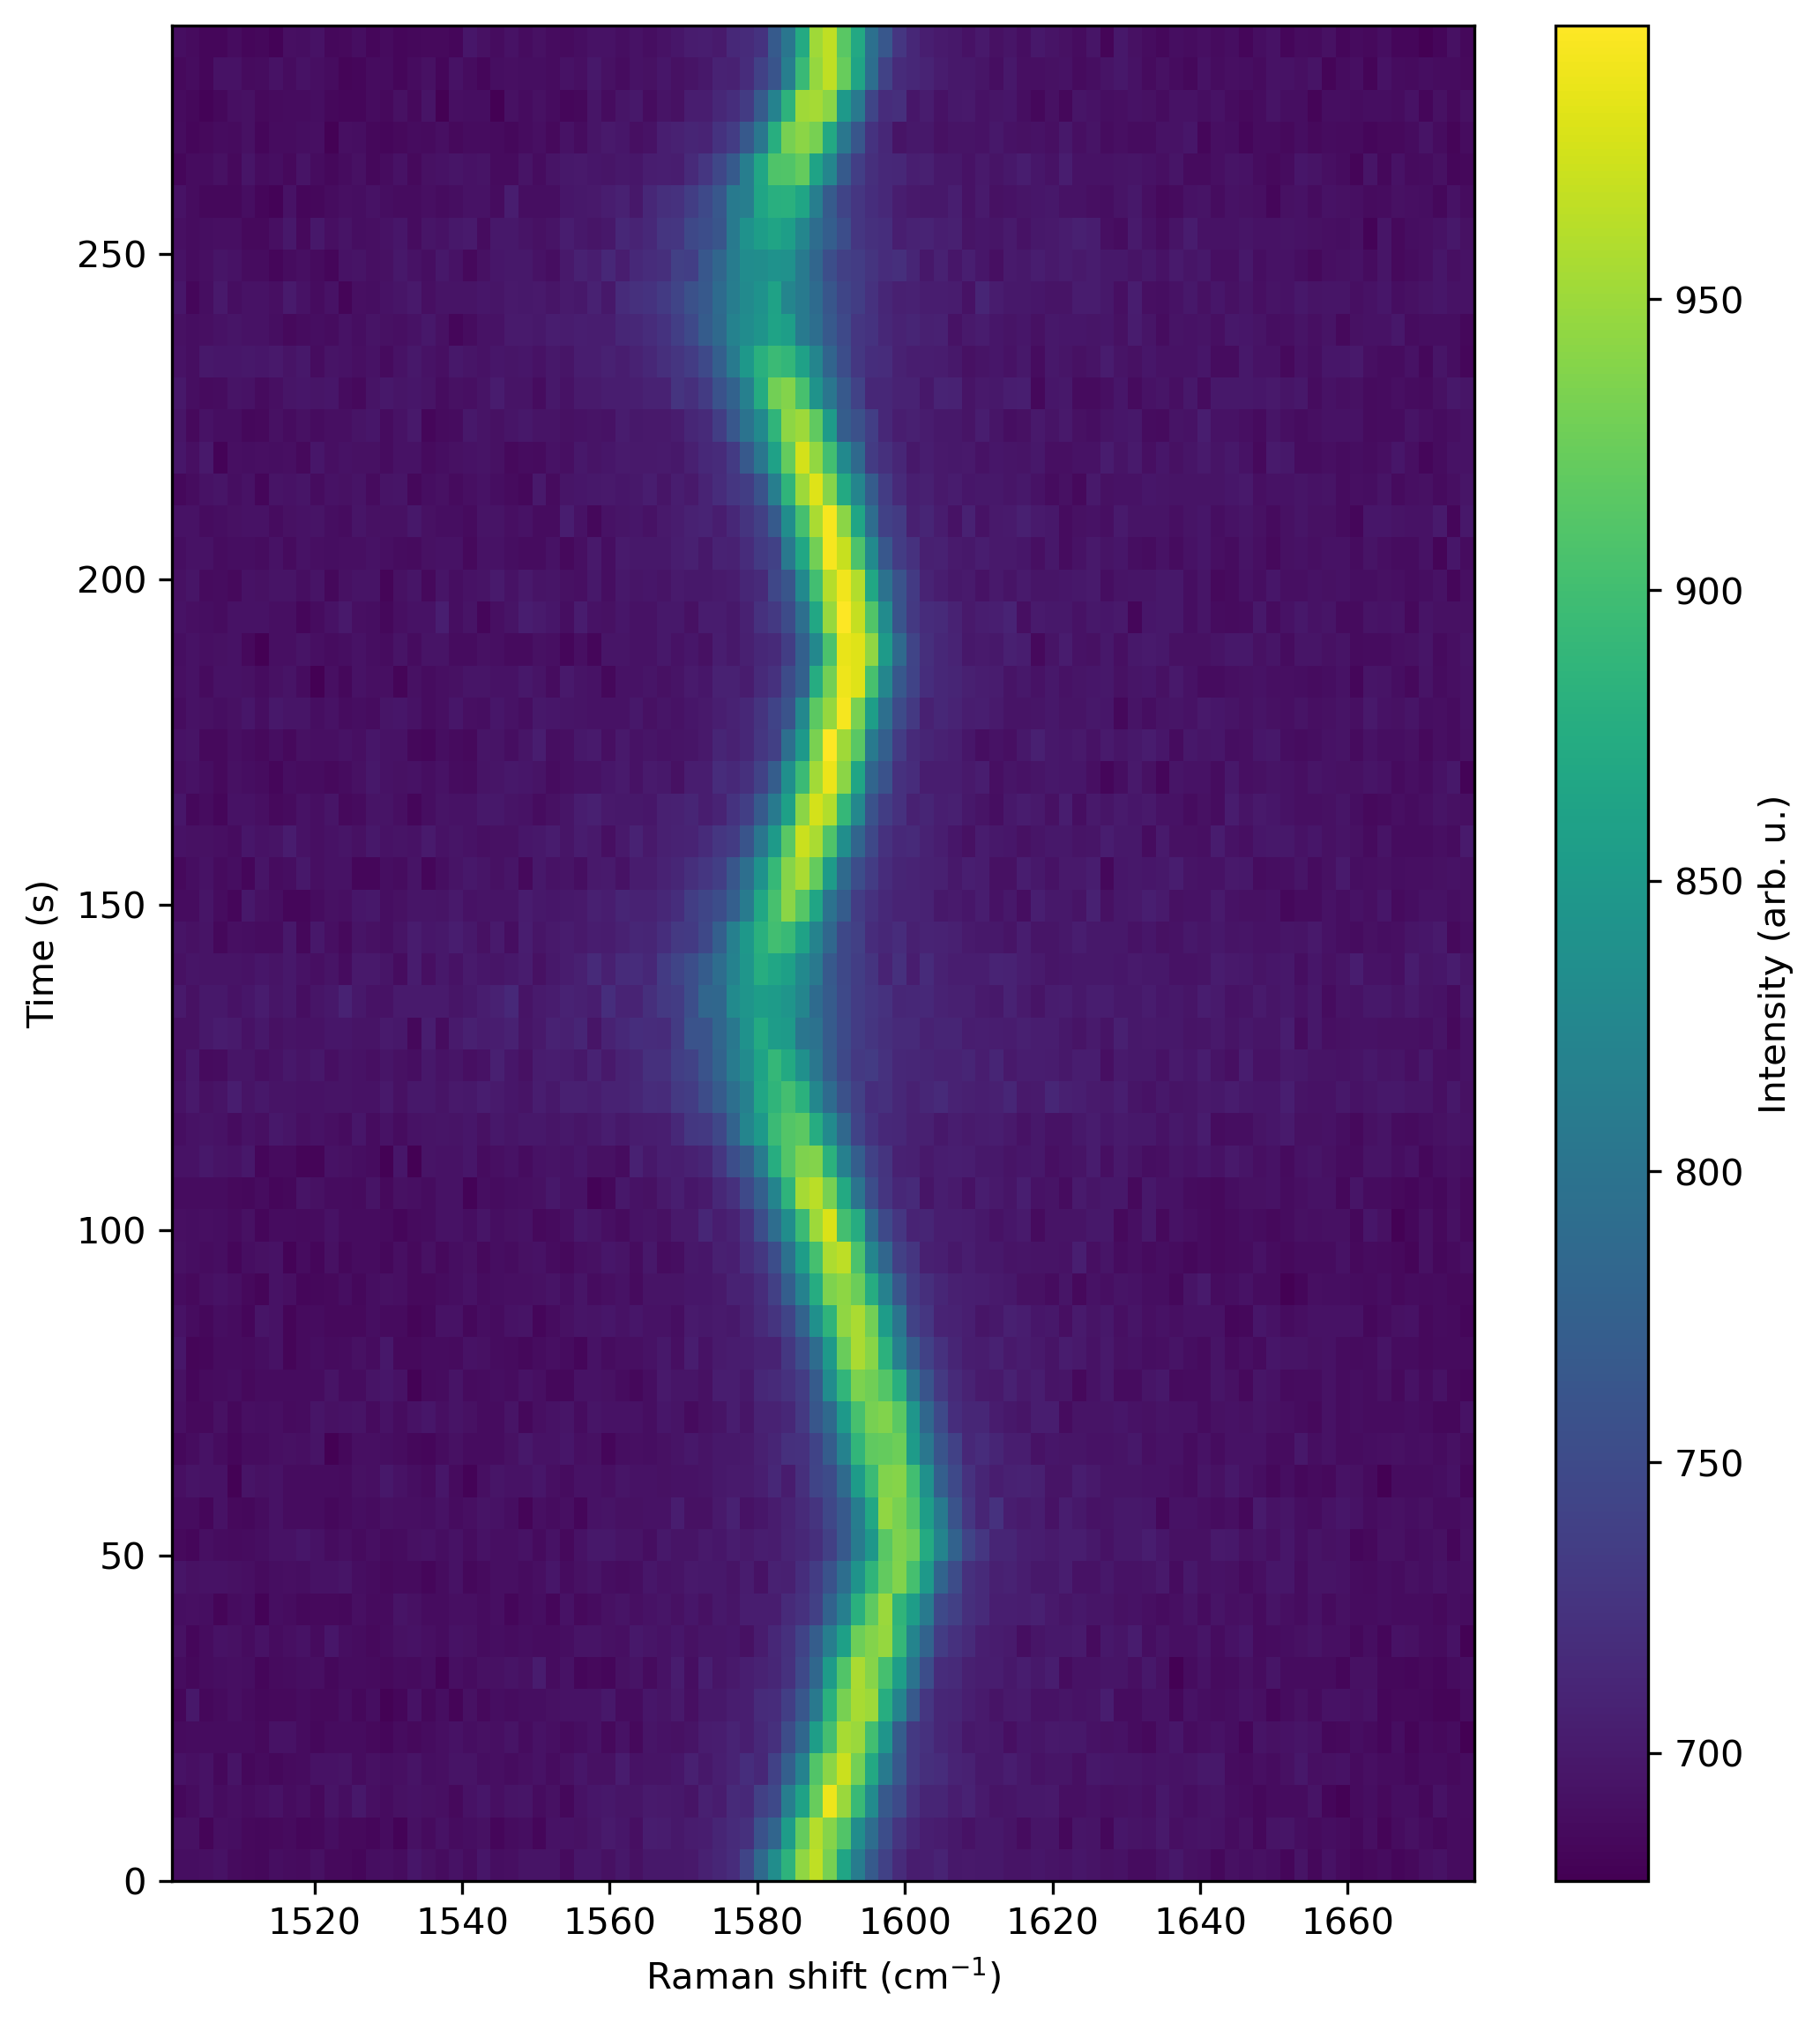
\includegraphics[width=0.5\linewidth]{Resources/heatmap_1D.png}
    \caption{Example of timescan mesurement in a form a heatmap}
    \label{heatmap_1D}
\end{figure}

An additional capability provided by this heatmap environment is the option to plot the spectrum directly onto the Main window. To enable this feature, simply perform a right-click on the desired spectrum image that you wish to examine thoroughly, and then choose the "Plot in Main" option from the context menu.

\subsection{Lineplot}
Another way to present a 1D Raman map is through a line plot. This method displays the spectra as a line plot with an offset determined by the slider. The slider adjusts the offset based on a percentage of the dataset's maximum intensity, making it dependent on the correction settings. The spectra are subsequently color-coded according to their indices. In this case, by right-clicking and choosing "Select region," only the spectral range will be selected. The exclusion of the indexes must be performed manually.

\begin{figure}[H]
    \centering
    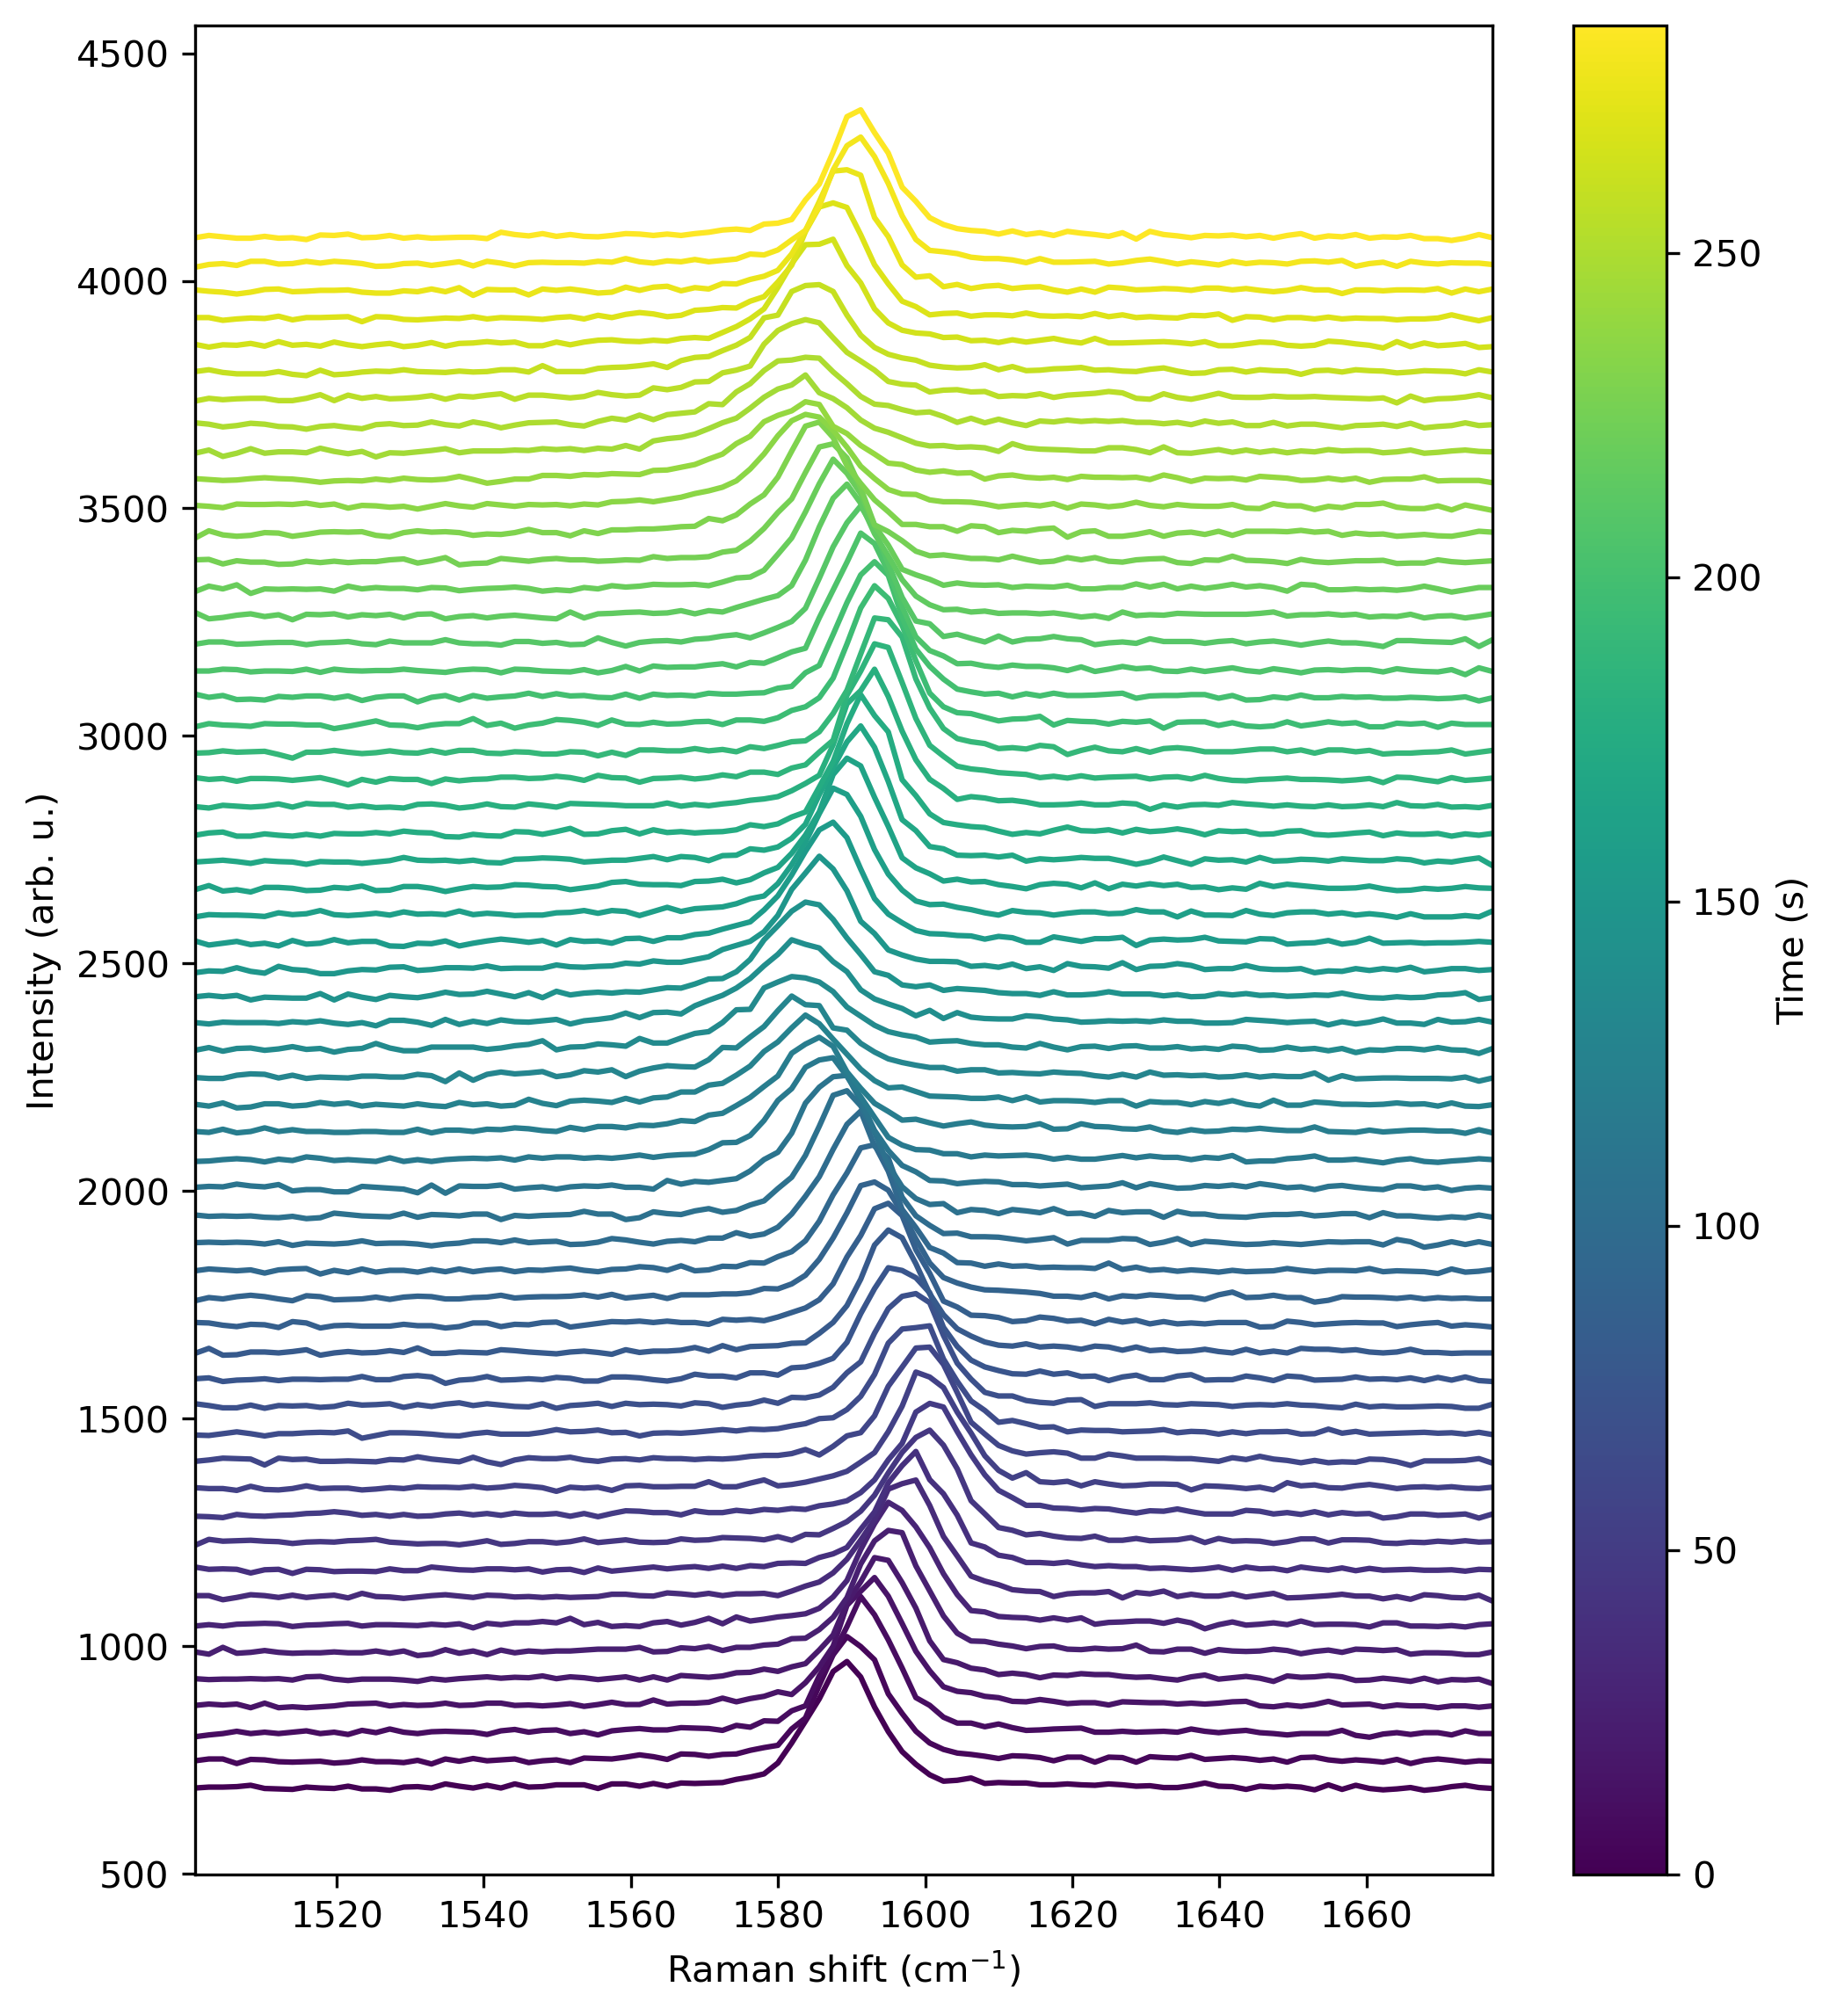
\includegraphics[width=0.5\linewidth]{Resources/lineplot_1D.png}
    \caption{Example of timescan mesurement in a form a lineplot}
    \label{lineplot_1D}
\end{figure}

\subsection{Fitting of the 1D map}
The Fit button triggers the fitting process for the one-dimensional map across the specified spectral range using the composite model set in the main window. In case a model is not yet specified, you may export the spectrum from the heatmap to the main window, where you can either manually define the model or import it from an existing .json file. Once the fitting process concludes, the resulting fit parameters and their corresponding indices are saved into an Excel file.

\section{2D mapping}
2D Raman mapping is a procedure in which Raman spectra are measured at different points on a surface, creating a two-dimensional map. Each pixel at this map represents a Raman spectrum, providing detailed information about the sample at each location.
Currently this app can analyses only the maps from Witec spectrometer, exported as table with header where columns contains the information about the pixel position (automatic export in Project5/6).

Loading of the Horiba 2D maps will be added in the future.

In the upper segment of the right column, just beneath the loading button, users can specify the map parameters. This includes defining the spectral region intended for analysis, along with setting the x and y range, allowing for analysis restricted to a specific part of the map. The spectral region requires manual setting; however, the x and y limits can be set by right-clicking on the map, selecting the "Select region" option, and then using a left-click to designate the desired area on the map. This function becomes particularly advantageous when a map is already displayed.

\subsection{Metric evaluation}
The initial assessment of the map involves computing the pixel metric. At this point, users have the option to choose among three metrics: the area (which refers to the integration of the spectrum area within a chosen spectral region), the maximum value (indicating the highest data value found within that spectral region), and max\_position (which denotes the spectral location of this maximum value). To display the metric map, you need to click on the "Plot metric" button. Additionally, there are other parameters you can adjust: the "Colormap," which specifies the color palette for the map, and "Interpolation," similar to its application in a 1D heatmap. You have the option to focus on a specific region of the evaluated parameter by setting the Scale's minimum and maximum values. This approach can help highlight particular data trends. Any values exceeding the set maximum or falling below the minimum will appear as saturated pixels, with their colors corresponding to either the top or bottom of the chosen color scale. Once the metric analysis is done, it does not need to be run again unless the spectral region is changed. If the spectral range is changed, the program will automatically detect it and run the new metric analysis after the next "Plot metric" click.

\subsection{Fitting of the 2D map}
To fit the 2D map, it is essential to have the model loaded in the main window, which will be used for fitting. There are multiple approaches to achieve this. If you're analyzing known spectral features, you might already have a .json file containing the model from previous work. In that situation, simply load the .json model into the main window. If the model isn't available, you can manually build it in the main window. You can export the spectrum from a single pixel or the map's average by right-clicking on the map and choosing "Plot spectra in Main" or "Plot average in Main." It is necessary to create the metric map first to have some data to export.

Once the model setup is complete, pressing the "Fit" button initiates the fitting process. When it is finished, the options for plotting the fit variables become accessible. Simply select the desired variable to plot from the "Fit variable" dropdown menu, which is pre-filled with variables from the model used, and then click on the "Plot fit" button. The other configurations of the map are the same as those for the Metric map.

The fitted values can be saved as an excel file for later use using the button "Save fit".

\section{Excel plotter}
The primary function of this feature is to swiftly allow for the visualization of map and batch fitting outcomes. Once the Excel file is loaded, users can effortlessly choose the data sources for both the x and y axes, assign appropriate labels, and proceed to create the plot. Assigning a third variable to define a color gradient is optional. Example of such plot could be seen in figure \ref{excel_plot}.

\begin{figure}
    \centering
    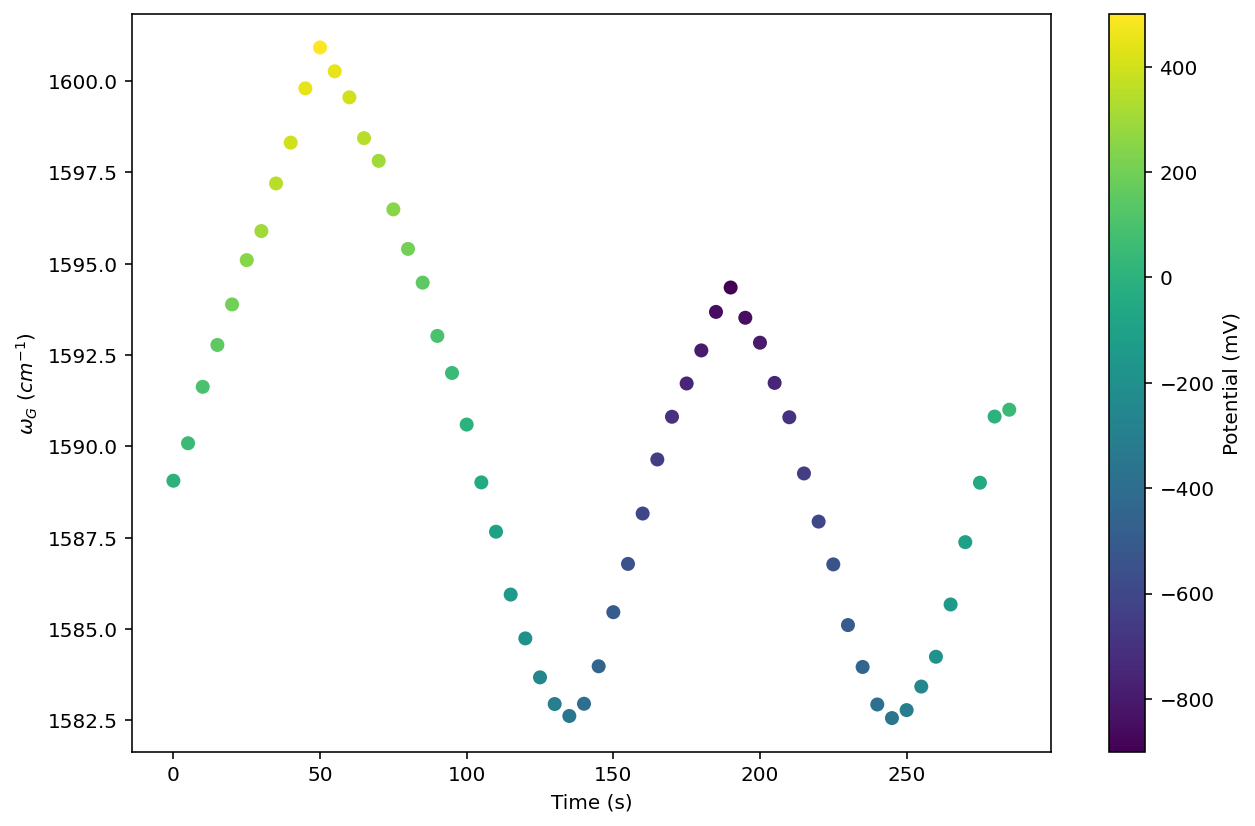
\includegraphics[width=0.75\linewidth]{Resources/Excel_plot.png}
    \caption{Example of plot made with "Excel plotter" enviroment}
    \label{excel_plot}
\end{figure}

\section{Principal Component Analysis}

The PCA module (Principal Component Analysis, powerful multivariate statistical technique) enables users to perform statistical decomposition of spectral datasets to identify and quantify underlying sources of variance — such as changes in doping, strain, chemical composition, or other sample properties — that may not be immediately evident in raw Raman or electrochemical spectra. Within the GUI, the process is designed to be straightforward and fully automated while retaining full scientific control over the analysis parameters.

\begin{figure}[H]
    \centering
    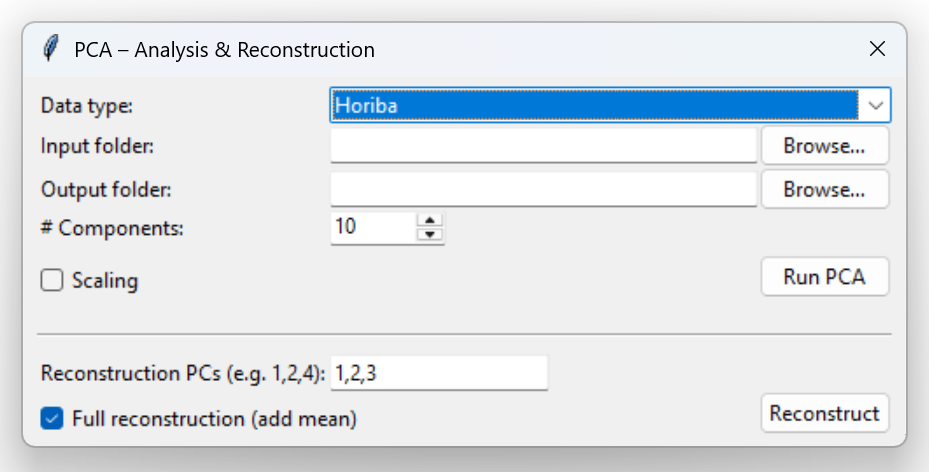
\includegraphics[width=0.75\linewidth]{Resources/PCA_env.png}
    \caption{Caption of the PCA setting enviroment}
    \label{PCA_env}
\end{figure}

The typical workflow begins by selecting a folder containing input spectra (in plain text format) and defining an output directory where all PCA results will be stored. The user can specify the number of principal components (PCs) to compute, as well as whether the data should be scaled (standardized to unit variance) or only mean-centered prior to decomposition. Once these options are set, pressing Run PCA will perform the analysis across all spectra in the selected folder.

Upon completion, the module automatically generates and saves a scree plot (showing the explained variance of each component), an Excel file containing the score values, and plots of score correlations between PC pairs to visualize clustering or sample evolution. The loading vectors are also saved — both as individual text files (matching the original spectral format) and as corresponding loading plots, allowing direct interpretation of which spectral regions contribute most to each component. All outputs are organized in the chosen output directory for traceability and further inspection.

\begin{figure}[H]
    \centering
    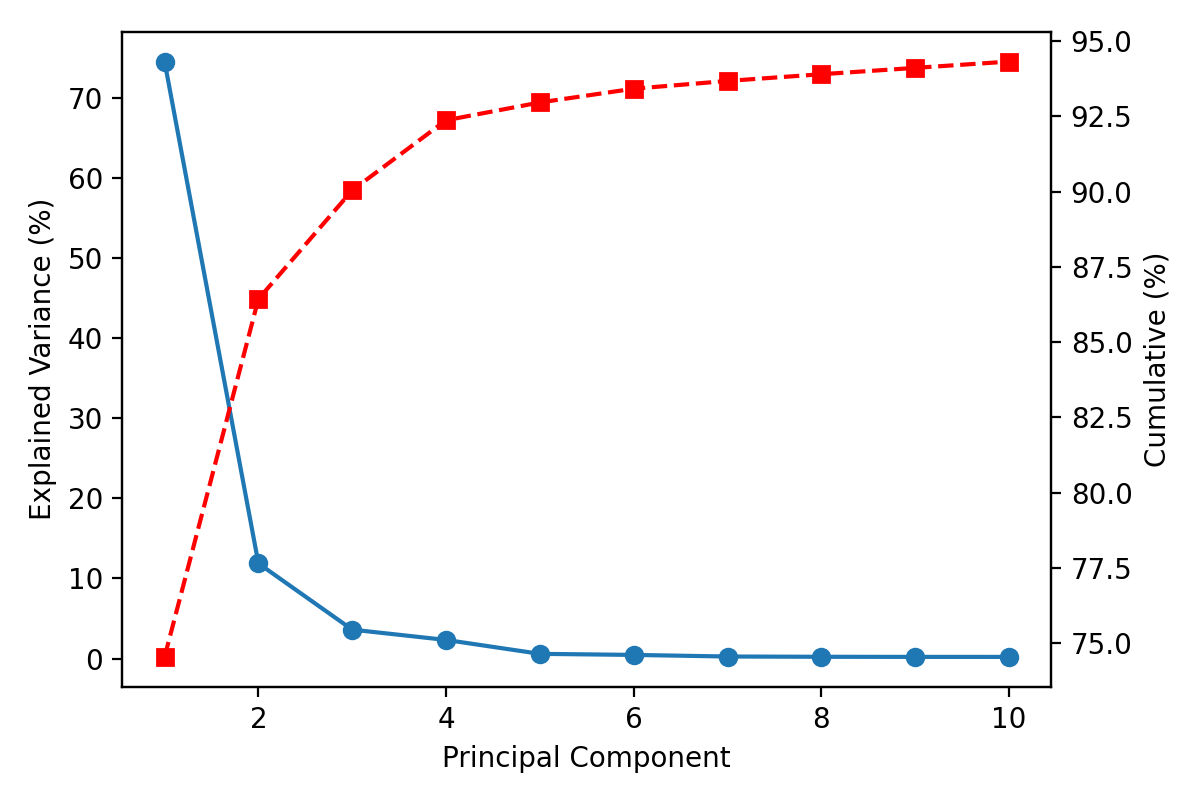
\includegraphics[width=0.5\linewidth]{Resources/scree_plot.png}
    \caption{Scree plot showing Explianed variance and Cumulative variance}
    \label{scree_plot}
\end{figure}

A dedicated reconstruction window allows users to selectively rebuild spectra using only chosen principal components, rather than a fixed variance threshold. This makes it possible to isolate the spectral contribution of specific components and visualize their effect on the overall dataset. The reconstruction can be performed either with the mean vector included (yielding the best approximation of the original spectra) or without the mean to highlight only the pure influence of the selected PCs on the spectral shape or intensity.

\begin{figure}
    \centering
    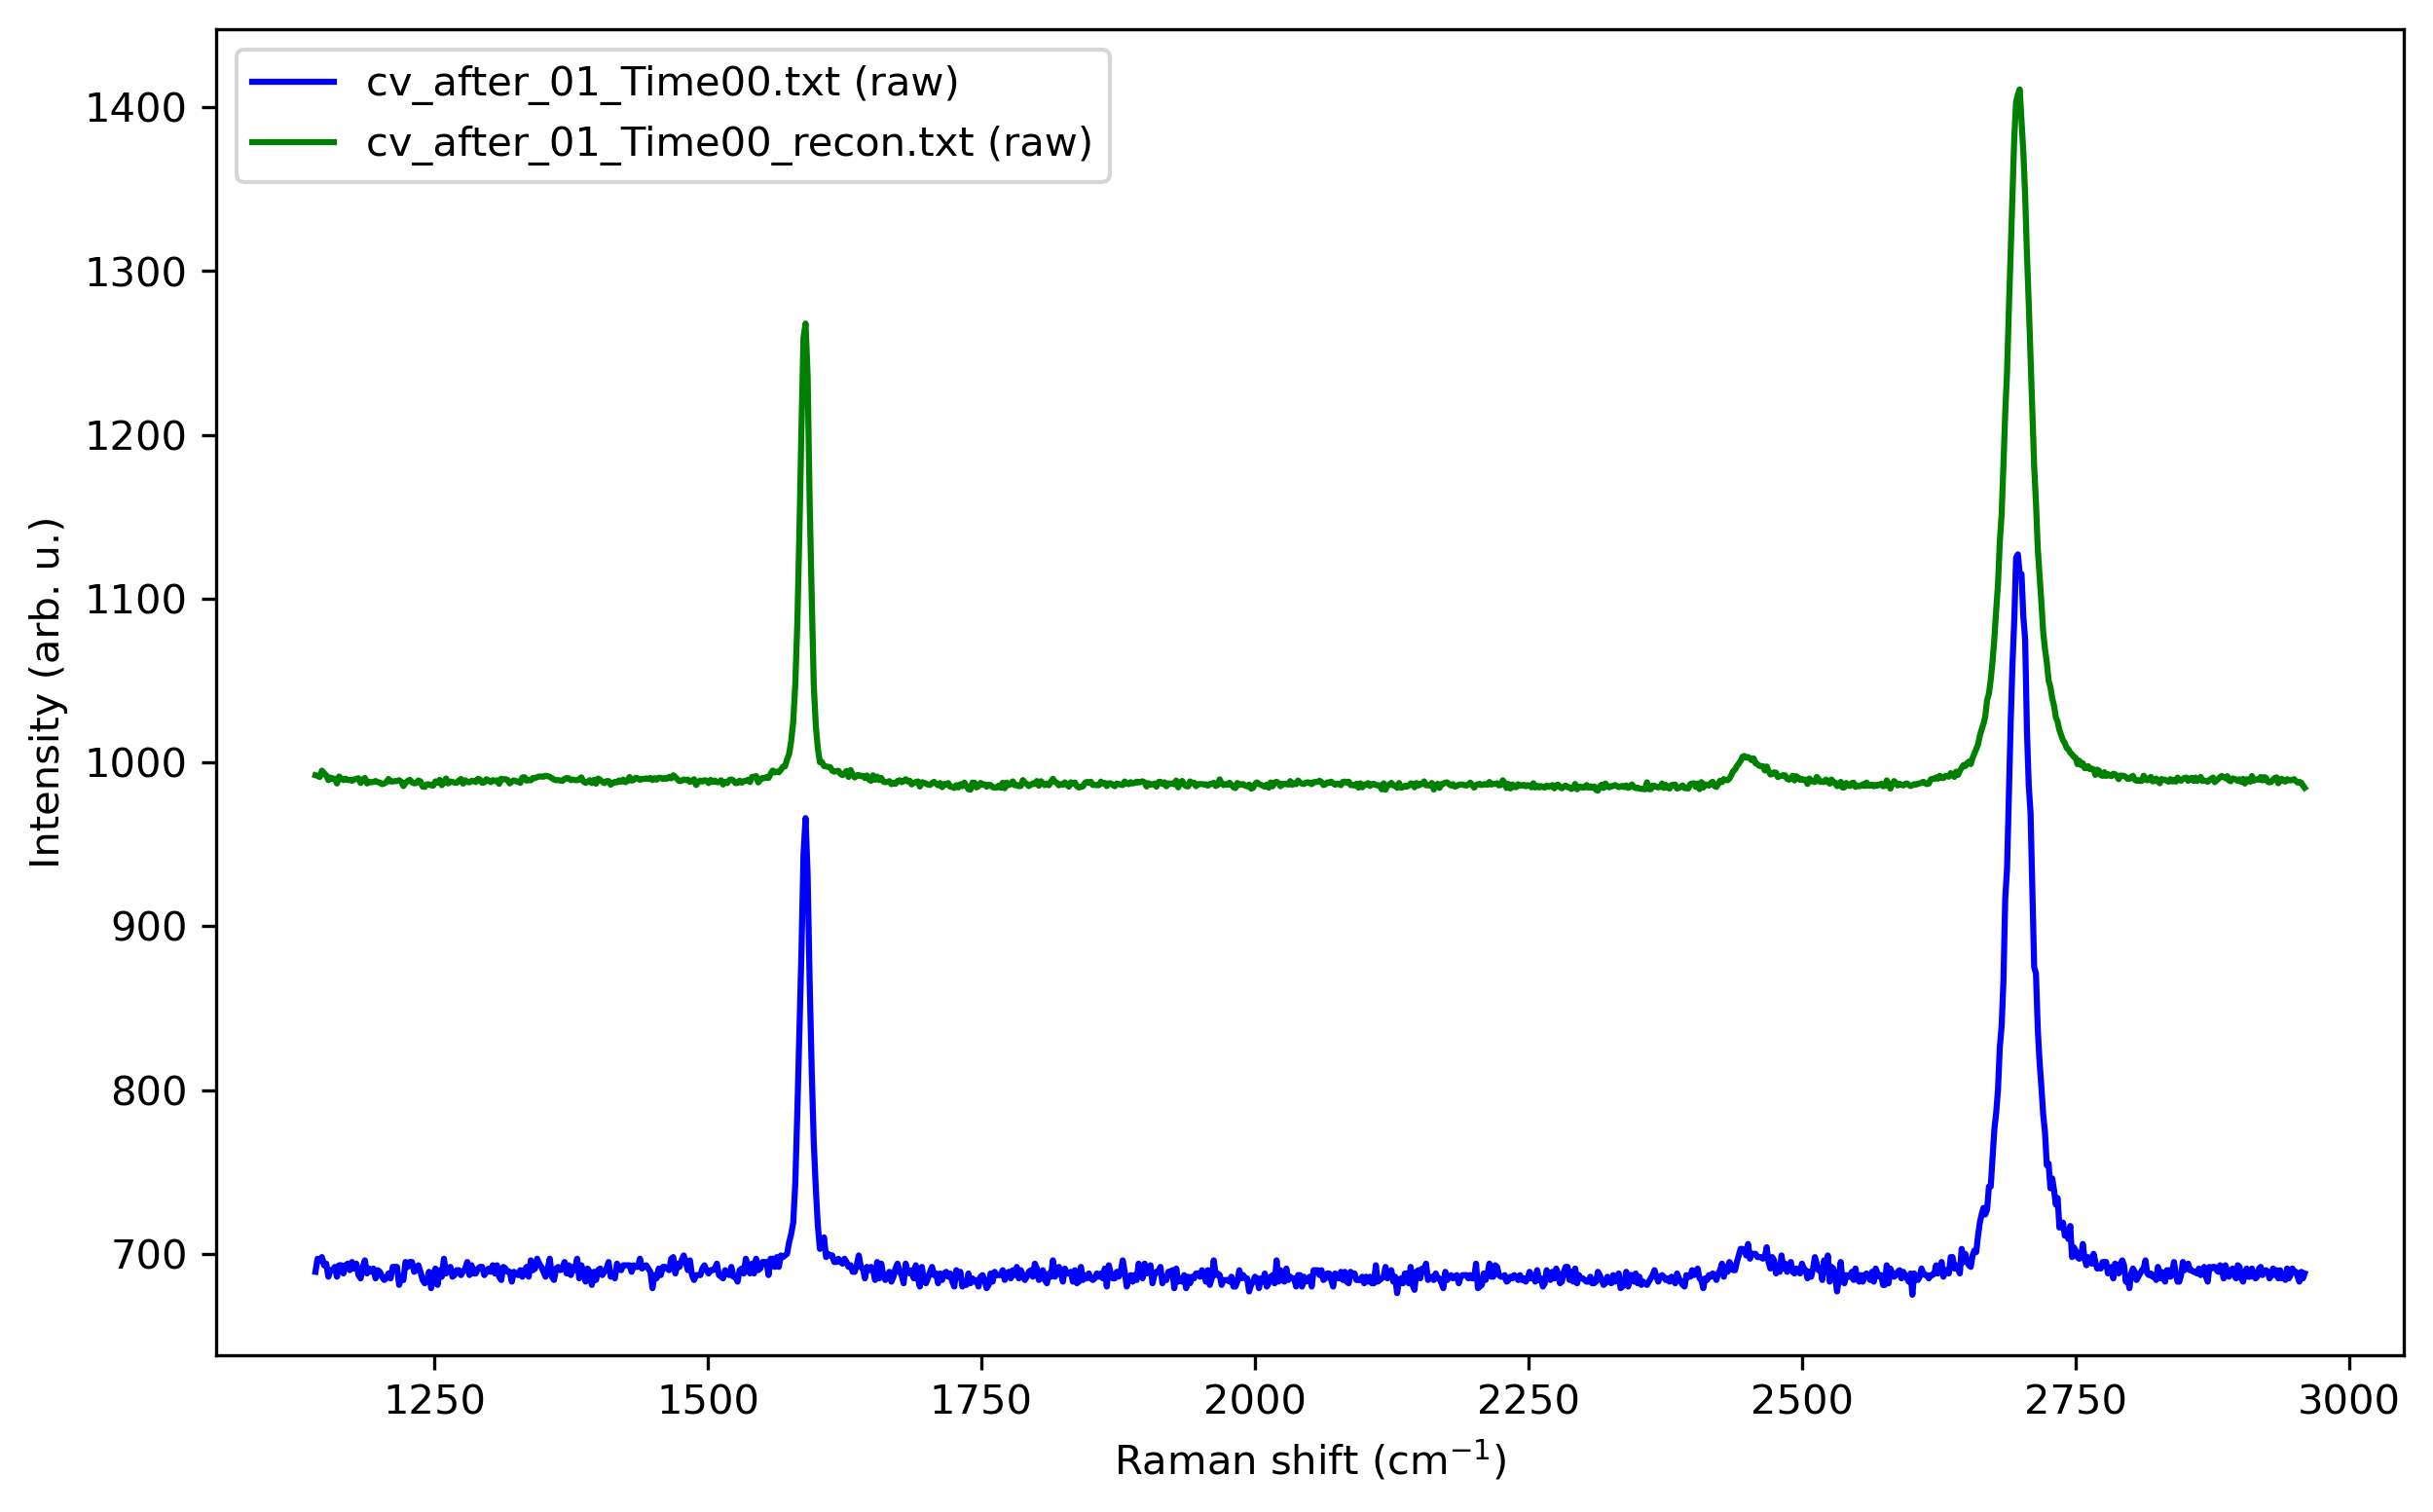
\includegraphics[width=0.75\linewidth]{Resources/00_compare.png}
    \caption{Comparison of original spectrum (blue) and reconstructed spectrum with only first three principal component (green)}
    \label{recon_compare}
\end{figure}

Importantly, once a PCA calculation has been completed, the entire model — including scores, loadings, mean vector, and metadata — is saved in a dedicated PCA result file (pca\_model.npz) located in the output folder. This allows the user to perform reconstructions later without repeating the full computation, simply by selecting the folder containing the saved PCA result file as the output directory. This ensures both reproducibility and flexibility, enabling efficient comparison of different reconstruction settings or datasets even after the main PCA run has been completed.

\subsection{Recommended workflow}

\begin{itemize}
    \item Open the PCA module from the main application window.
    \item Select input folder containing the spectral data files (e.g., .txt spectra with identical Raman shift axes).
    \item Select output folder where all PCA results and plots will be saved.
    \item Set the number of components (N PCs) to compute — typically between 5 and 20 depending on dataset complexity.
    \item Choose preprocessing options:
    \begin{itemize}
        \item Scaling: Normalize each variable to unit variance (recommended when absolute intensities differ greatly).
        \item No scaling: Apply only mean-centering (recommended when absolute intensities carry physical meaning).
    \end{itemize}
    \item Run PCA computation.
    \item The app will automatically:
    \begin{itemize}
        \item Save the scree plot showing explained variance ratios.
        \item Export scores as an Excel file and score correlation plots for PC combinations.
        \item Save loading vectors both as .txt files and as corresponding loading plots.
    \end{itemize}
    \item Perform reconstruction (optional):
    \begin{itemize}
        \item Choose any subset of PCs to rebuild spectra.
        \item Decide whether to include the mean vector (for full-spectrum reconstruction) or exclude it to visualize only the isolated spectral effect of selected components.
    \end{itemize}
    \item Reopen results later:
    \begin{itemize}
        \item Each PCA run generates a dedicated PCA result file stored in the output folder.
        \item You can load this file later to perform reconstructions or comparisons without re-running PCA on the raw data.
    \end{itemize}
\end{itemize}